\section{Colored Gaussian Noise Channels}
Considering Channels whose Noise is dependent on one another , which can be seen as a blend of parallel channels along with gaussian channels with memory including noise.
\\
Considering $n$ parallel gaussian channels whose noise is dependent , considering the input covariance matrix of input and noise to be $K_x$ and $K_z$ respectively. The power constaint of input now depends on $n$ and can be seen as,
\begin{equation}
\frac{1}{n} \sum_i \mathbb{E}X_i^2 \leq P,
\tag{10.77}
\end{equation}
(or)
\begin{equation}
\frac{1}{n} \operatorname{tr}(K_X) \leq P.
\tag{10.78}
\end{equation}
Channel Capcity can be written same as before , $ie$:
\begin{equation}
I(X_1, X_2, \ldots, X_n ; Y_1, Y_2, \ldots, Y_n) = h(Y_1, Y_2, \ldots, Y_n) - h(Z_1, Z_2, \ldots, Z_n).
\tag{10.79}
\end{equation}

The choice of input distribution does not affect \( h(Z_1, Z_2, \ldots, Z_n) \) where as it is dependent on distribution of the noise.Hence, maximizing \( h(Y_1, Y_2, \ldots, Y_n) \) maximizes capacity.
When the input is normal and \( Y \) is normal , it is said to maximize the entropy of the output.
\\
The Covariance of the output \( Y \) since the input and the noise are independent can be given by \( K_Y = K_X + K_Z \) and the entropy is
\begin{equation}
h(Y_1, Y_2, \ldots, Y_n) = \frac{1}{2} \log((2 \pi e)^n |K_X + K_Z|).
\tag{10.80}
\end{equation}
To maximise \( |K_X + K_Z| \) , we need to carefully choose \( K_X \). For that taking diagonal form of \( K_Z \) ,
\begin{equation}
K_Z = Q \Lambda Q^T, \quad \text{where } Q Q^T = I.
\tag{10.81}
\end{equation}
Then
\begin{align}
|K_X + K_Z| &= |K_X + Q \Lambda Q^T| \tag{10.82} \\
&= |Q| |Q^T K_X Q + \Lambda| |Q^T| \tag{10.83} \\
&= |Q^T K_X Q + \Lambda| \tag{10.84} \\
&= |A + \Lambda|, \tag{10.85}
\end{align}
where \( A = Q^T K_X Q \).
\\
It is known that the trace is same and is independent of the order of multiplication,
\begin{equation}
\operatorname{tr}(BC) = \operatorname{tr}(CB),
\tag{10.86}
\end{equation}
we have
\begin{equation}
\operatorname{tr}(A) = \operatorname{tr}(Q^T K_X Q),
\tag{10.86}
\end{equation}
%
Changing the order of RHS,
\begin{equation}
\operatorname{tr}(A) = \operatorname{tr}(QQ^T K_X )
\tag{10.86}
\end{equation}
%
since $QQ^T = 1$ we get, 
\begin{equation}
\operatorname{tr}(A) = \operatorname{tr}( K_X )
\tag{10.86}
\end{equation}
%
Within the constraint \( \operatorname{tr}(\mathbf{A}) \leq nP \) , we need to maximise \( |\mathbf{A} + \mathbf{\Lambda}| \) .
%
\begin{tcolorbox}[boxrule=0pt,frame hidden,sharp corners,enhanced, opacityback=0, borderline west={2pt}{0pt}{red}]
\begin{defn} \textbf{(Hadamard's Inequality)} Hadamard's inequality states that product of its diagonal elements is greater than determinant of any non-negative matrix \( \mathbf{K} \)  i.e.,
\begin{equation}
|\mathbf{K}| \leq \prod_i K_{ii}
\end{equation}
with equality if and only if the matrix is diagonal.
\end{defn}
\end{tcolorbox}
%
Applying Hadamard's inequality here,
\begin{equation}
|\mathbf{A} + \mathbf{\Lambda}| \leq \prod_i (A_{ii} + \lambda_i)
\tag{4.1}
\end{equation}
with equality if \( \mathbf{A} \) is diagonal. 
\newpage
Getting the power constraint on \( \mathbf{A} \),
\begin{equation}
\frac{1}{n} \sum_i A_{ii} \leq P,
\end{equation}
and since \( A_{ii} \geq 0 \), 
\\
$RHS$ of $eq$ $4.1$ has the maximum value when
\begin{equation}
A_{ii} + \lambda_i = \nu.
\end{equation}
Sometimes , we might not be able to statisfy the equation due to the constriants given above with non-negative \( A_{ii} \).
Kuhn-Tucker conditions can be used to find the optimum solution for value of \( \nu \)
\begin{equation}
A_{ii} = (\nu - \lambda_i)^+,
\end{equation}
where \( \nu \) is such that \( \sum_i A_{ii} = nP \). 
\\
Entropy of Y gets maximized based on value of \( \mathbf{A} \), which lads to the goal of maximizing the channel capacity.
\\
Methods discussed here can be seen to be similar to $"Water-Filling"$ process discussed in the previous section of the paper.
If there is a channel whose noise is forming a stochastic process with finite dimensional covariance matrix \( K_x^n \) given that the noise in the channel is a additive Gaussian noise .Then the eigenvalues of \( K_x^n \) tend to a limit of \( n \to \infty \).
Power spectrum of such a stochastic process is described by the density of eigenvalues and the similarity to $"Water-Filling"$ process can be described in the terms of spectral domain and graphical representation can be seen as below.
\begin{center}
	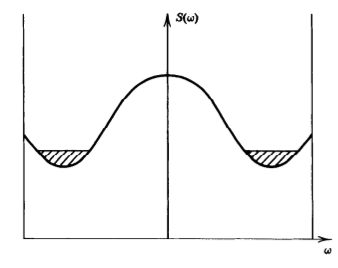
\includegraphics[scale=0.5]{Diagrams/water_filling_spectral_domain.png}
\end{center} 
It can be concluded that for noise in channels which forms a stationary stochastic process, choosing a input signal is critical , it has to be a Gaussian process whose noise spectrum is small , and its input signal spectrum is large at frequencies. 
\\
For a Channel which has Additive Gaussian Noise , and whose power spectrum of Noise is described as $N(f)$ , the capacity is given by:
\begin{align}
C &= \frac{1}{2} \log \left( 1 + \frac{\nu - N(f)^*}{N(f)} \right) \,\mathrm{d}f
\end{align}
and value is $\nu$  such  $\int (v - N(f))^* \,\mathrm{d}f = P$ satisfies.